To experimentally validate the thermal performance of the two winding orientations, representative physical prototypes of the edgewise-wound and flatwise-wound transformers were fabricated. This section details the thermal performance comparison of the proposed and conventional-wound structures under steady-state operation in full load by examining key spots in the transformers. Moreover, the system-level efficiency with the two transformers is also quantified.
\section{Prototype Construction}
Representative physical prototypes of the edgewise-wound and flatwise-wound transformers were fabricated. To ensure a direct geometric comparison, Tr2E and Tr2F were selected as the edgewise-wound and flatwise-wound prototypes since they feature a square window area. The manufactured edgewise-wound prototype for Tr2E and its cross-section is shown in Figures \ref{fig:edgewise_3D} and \ref{fig:edgewise_cross} respectively. The manufactured flatwise-wound prototype for Tr2F and its cross-section is shown in Figure \ref{fig:flatwise_3D} and Figure \ref{fig:flatwise_cross} respectively. 

\begin{figure}[h!]
    \centering
    \subfloat[]{
        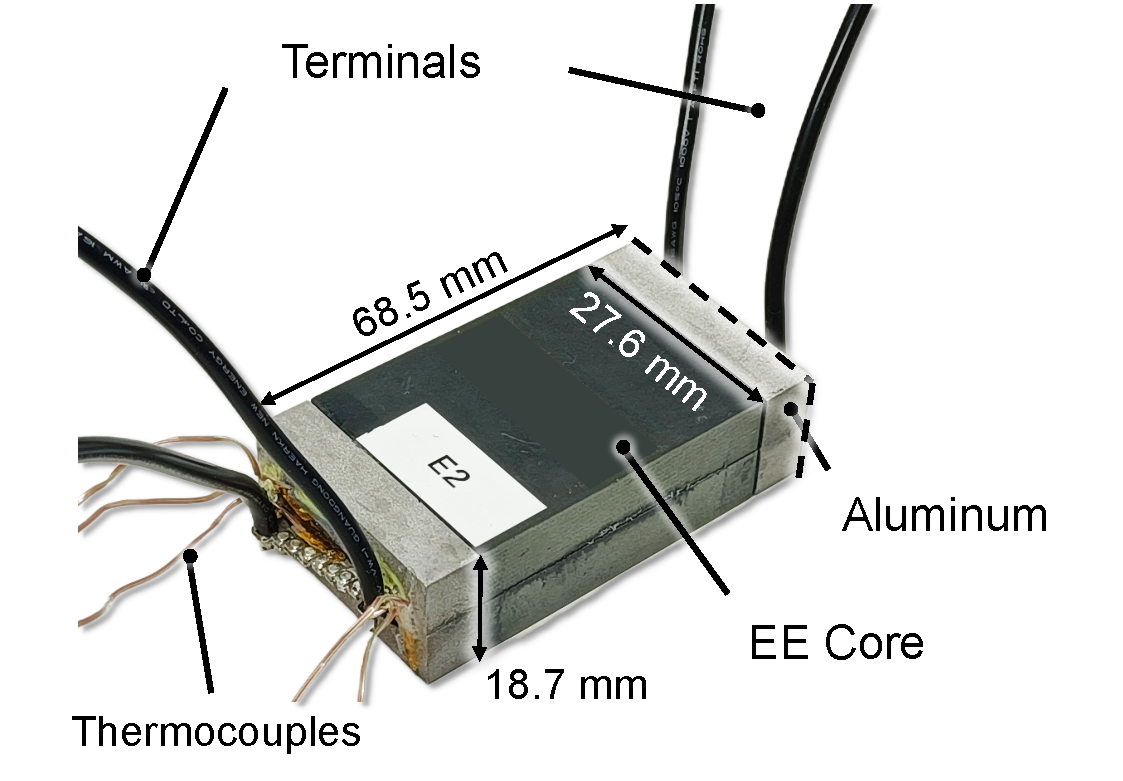
\includegraphics[width=0.5\columnwidth]{figures_chapter5/edgewise_3D_prototype.pdf}%
        \label{fig:edgewise_3D}
    }
    \subfloat[]{
        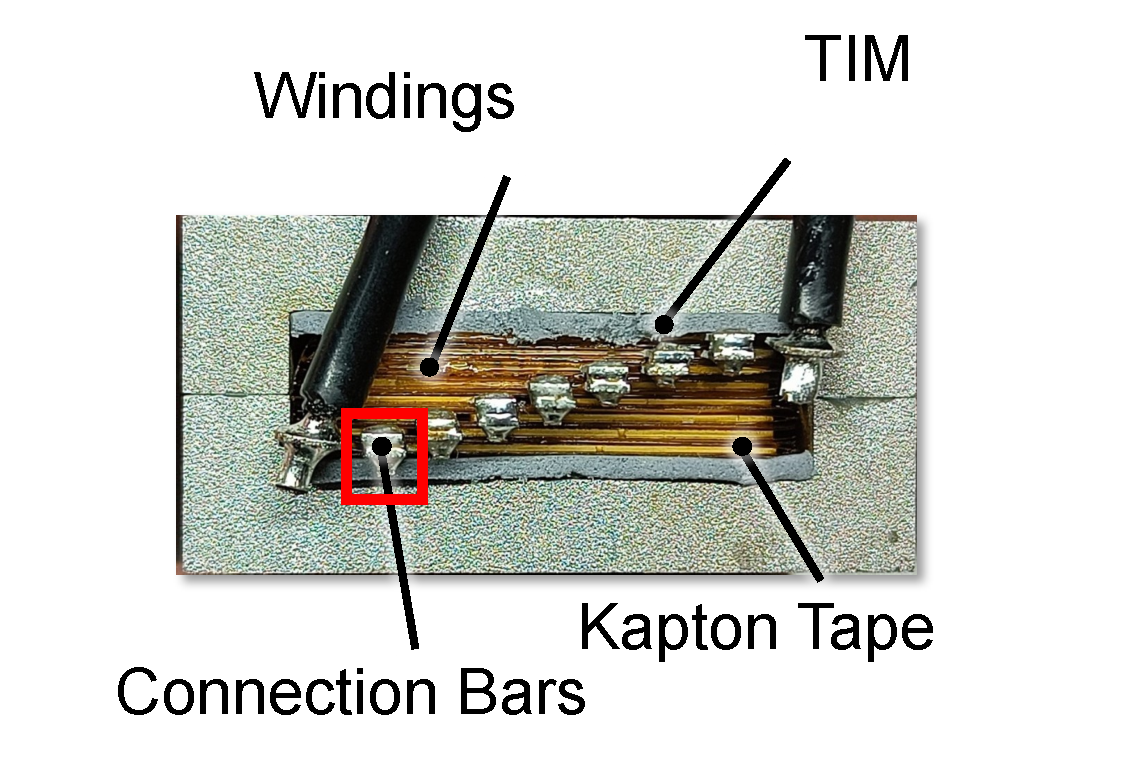
\includegraphics[width=0.5\columnwidth]{figures_chapter5/edgewise_cross_prototype.pdf}
        \label{fig:edgewise_cross}
    }
    \caption{(a) Prototype edgewise-wound transformer representing Tr2E, (b) cross-section of the edgewise-wound transformer prototype. The manufacturing limitation of the prototype is shown with the red box.}
    \label{fig:edgewise}
\end{figure}

\begin{figure}[h!]
    \centering
    \subfloat[]{
        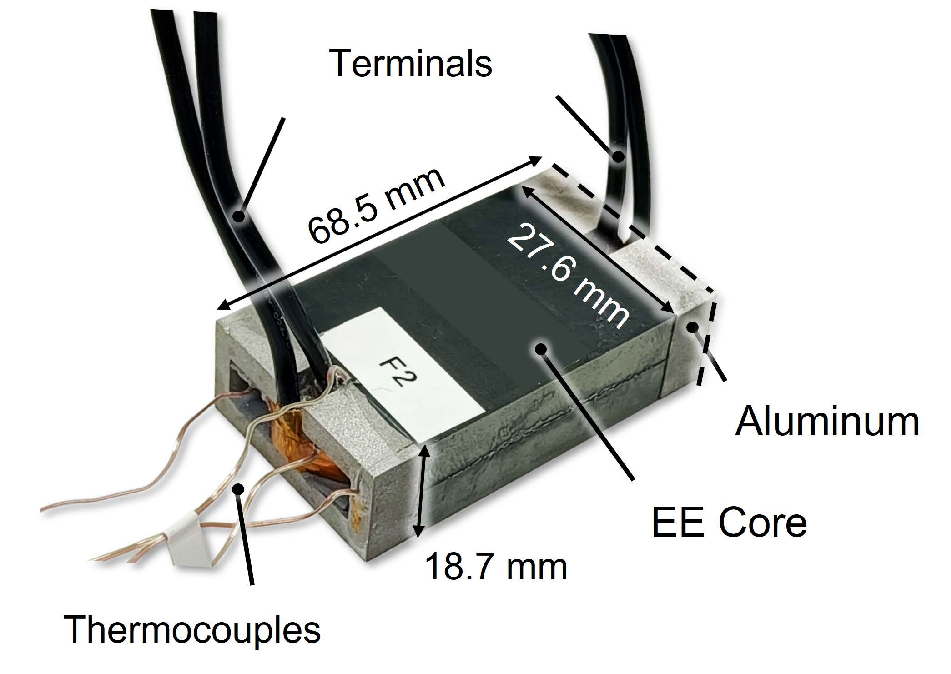
\includegraphics[width=0.5\columnwidth]{figures_chapter5/flatwise_3D_prototype.pdf}%
        \label{fig:flatwise_3D}
    }
    \subfloat[]{
        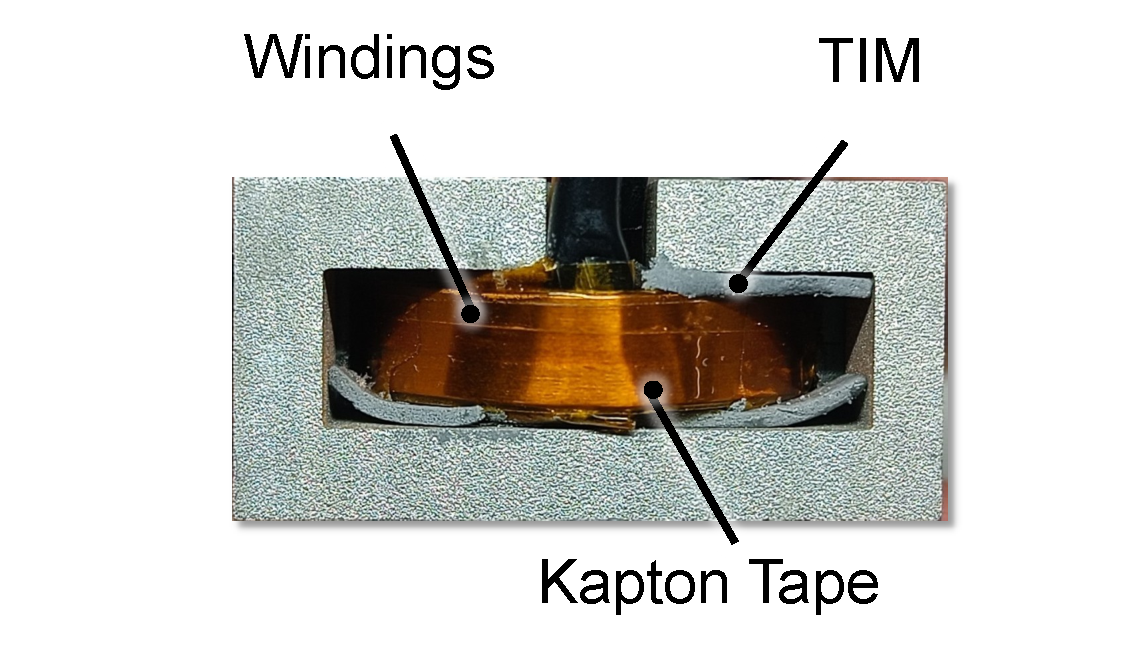
\includegraphics[width=0.5\columnwidth]{figures_chapter5/flatwise_cross_prototype.pdf}
        \label{fig:flatwise_cross}
    }
    \caption{(a) Prototype flatwise-wound transformer representing Tr2F, (b) cross-section of the flatwise-wound transformer prototype.}
    \label{fig:flatwise}
\end{figure}

Both prototypes utilize a custom-made LP10A ferrite EE-core with an air gap of 0.10 mm. To facilitate the supplementary heat extraction mechanisms defined in Section \ref{section:heat_dissipation}, DR-X100 (10 W/mK) was applied as the TIM between the core and the windings, and Al3031 aluminum blocks were fitted into the dead space. 

Several limitations arose during the fabrication of the prototypes. There were a few differences in the core dimensions and the wire dimensions as well due to the availability and capability of the custom manufacturability. 

For the conventional edgewise-wound transformer, strict spatial constraints dictated that the windings could not be continuously formed. Instead, the individual turn layers had to be connected and soldered in series using external connection bars that bridge the adjacent layers as shown in Figure \ref{fig:edgewise_cross}. For the flatwise-wound transformer, the continuous winding and folding process resulted in a curved profile at the bends as shown in Figure~\ref{fig:flatwise_cross}. This causes deviations in $d_\mathrm{clear}$ from the idealized simulated geometry. 

Furthermore, while the simulations modeled the inter-turn insulation solely as air, Kapton tape PF301 was applied to the physical windings to ensure dielectric safety in prolonged converter operation. Inherent assembly tolerances also introduced unintended changes in $d_{\mathrm{inter}}$ for both transformers, causing the turns to have unequal air gaps. These manufacturing steps naturally introduce physical imperfections compared to the idealized simulated designs, which are expected to cause deviations in the behaviors seen in the simulations. The detailed physical, magnetic, and electrical specifications at 28.5 kHz for each assembled transformer are summarized in Table \ref{tab:prototype_specs}.

\begin{table}[h!]
    \centering
    \caption{Specifications of the Prototype Transformers}
    
    \setlength{\tabcolsep}{3pt} % Reduces default space between columns
    \resizebox{\columnwidth}{!}{%
    \begin{tabular}{lccc}
    \hline
    \hline
    \textbf{Parameter} & \textbf{Symbol} & \textbf{Edgewise Prototype} & \textbf{Flatwise Prototype} \\
    \hline
    Magnetizing Inductance & $L_{\mathrm{m}}$ & 196.25 $\upmu$H & 196.97 $\upmu$H \\
    Conductor Dimensions & $w \times t$ & \multicolumn{2}{c}{6.00 $\times$ 0.30 mm}\\
    Number of Turns & $N_{\mathrm{p}} : N_{\mathrm{s}}$ & \multicolumn{2}{c}{8 : 8} \\
    Coupling Coefficient & $k$ & \multicolumn{2}{c}{0.9988} \\
    Air Gap & $l_{\mathrm{g}}$ & \multicolumn{2}{c}{0.10 mm} \\
    Window Area & $A_{\mathrm{win}}$ & {77.44 mm$^2$} & {76.56 mm$^2$} \\
    Window Aspect Ratio & $l_{\mathrm{win}}/w_{\mathrm{win}}$ & \multicolumn{2}{c}{$\sim$1.00} \\
    Transformer Dimensions & $l_{\mathrm{tr}} \times w_{\mathrm{tr}} \times h_{\mathrm{tr}}$ & \multicolumn{2}{c}{68.5 $\times$ 27.6 $\times$ 18.7 mm} \\
    Core Material & -- & \multicolumn{2}{c}{Ferrite LP10A} \\
    Core-to-Winding TIM & -- & \multicolumn{2}{c}{DR-X100 (10.0 W/(m$\cdot$K))} \\
    Dead Space Block & -- & \multicolumn{2}{c}{Al3031} \\
    \hline
    \hline
    \end{tabular}%
    }
    \label{tab:prototype_specs}
\end{table}

\section{Experimental Setup}
\subsection{Thermal Evaluation Setup}
Thermocouples were embedded on both transformer prototypes to capture the spatial thermal distribution, as illustrated in Figure \ref{fig:thermocouple}. The measurement nodes were selected to provide a comprehensive thermal profile. Specifically, the targeted measurement points included: the winding temperature $T_{\mathrm{wind}}$; the internal core window temperatures at the top and left side, $T_{\mathrm{top, in}}$ and $T_{\mathrm{left, in}}$; the exterior core temperatures $T_{\mathrm{top, out}}$, $T_{\mathrm{left, out}}$, and $T_{\mathrm{bot, out}}$; and the dead-space aluminum block temperature $T_{\mathrm{Al}}$.

\begin{figure}[h!]
    \centering
        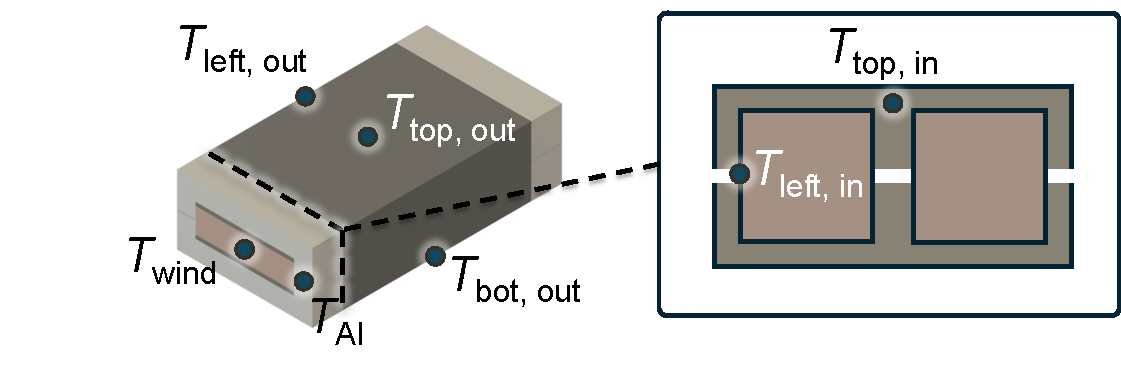
\includegraphics[width=0.85\columnwidth]{figures_chapter5/thermocouple.pdf}%
    \caption{Thermocouple placement for the measurement of key spots in the transformers. Thermocouples  $T_{\mathrm{left, out}}$, and $T_{\mathrm{bot, out}}$ are placed on the center of their respective faces as well.}
    \label{fig:thermocouple}
\end{figure}

Because the transformer geometry and internal heat generation are symmetric, thermocouple placement was concentrated on a single representative section to characterize the entire structure. This meant that the thermocouples on the respective internal and external faces indicated are placed on the center of their faces. The thermocouple for the winding was placed towards the middle, which meant between the fourth primary and secondary winding. The number of exterior sensors were minimized to prevent parasitic thermal mass and convection interference from skewing the thermal measurements. More insight into this is included in the Appendix: \nameref{app:longresult}.

The thermal evaluation was conducted under natural cooling and forced-air cooling through a heat sink. In the natural cooling setup depicted in Figure \ref{fig:natural}, the transformer was elevated on a wooden block. This low-thermal-conductivity boundary isolates the prototype by minimizing parasitic heat conduction through the bottom surface, ensuring that heat dissipation is only by natural convection to the surrounding ambient air. In the forced-air cooling configuration depicted in Figure \ref{fig:forcedair}, the transformers were physically coupled to an aluminum heatsink via a 1.00 mm TIM (ASKER C18 CPVS series, Kitagawa Industry Co., Ltd.) and subjected to active cooling from a 10.0-W fan. Across both test conditions, the thermal profiles were continuously recorded using a GRAPHTEC 200 data logger until an absolute thermal steady-state was achieved.

\begin{figure}[h!]
    \centering
    \subfloat[]{
        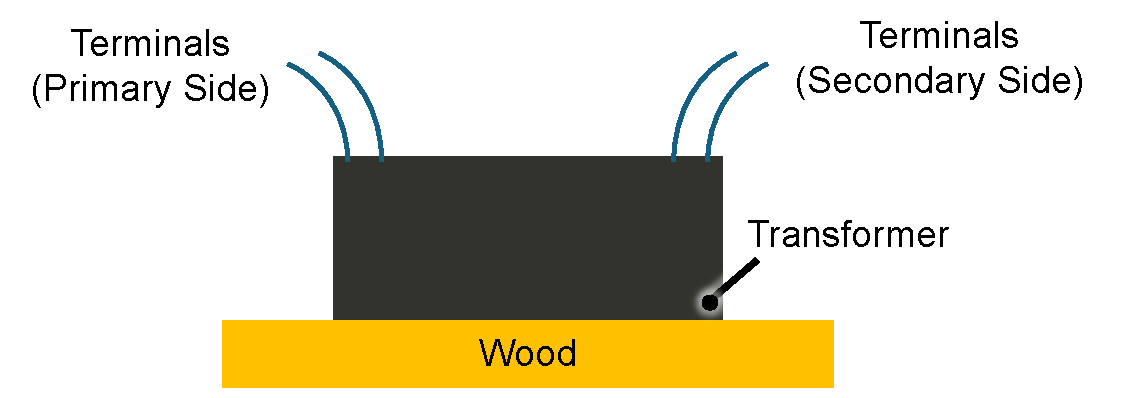
\includegraphics[width=0.8\columnwidth]{figures_chapter5/setup_natural.pdf}%
        \label{fig:natural}
    }

    \subfloat[]{
        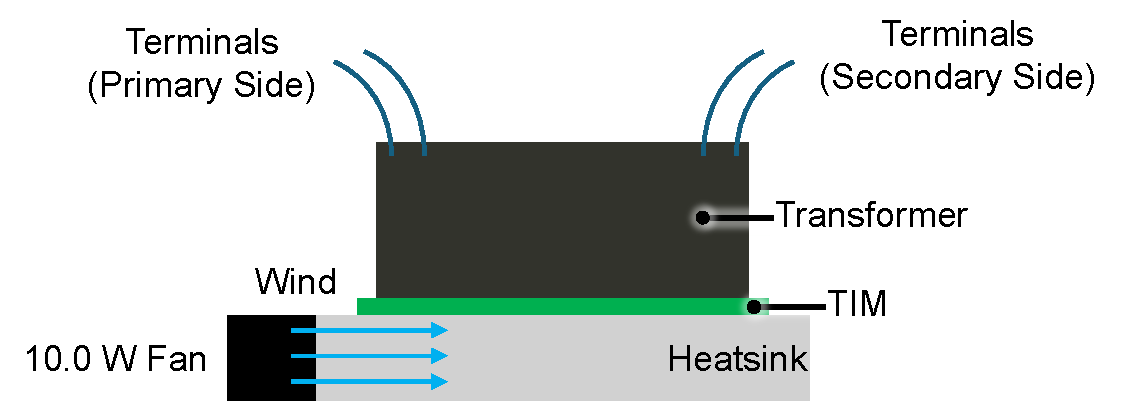
\includegraphics[width=0.8\columnwidth]{figures_chapter5/setup_forced.pdf}
        \label{fig:forcedair}
    }
    \caption{Cooling-setups for the transformers: (a) natural-cooling, (b) forced-air cooling through heat sink.}
    \label{fig:cooling setup}
\end{figure}
\pagebreak
\subsection{Experimental Environment and Implementation}
The prototyped transformers were evaluated in a 1-kW, 100-V CLLC converter operating at full load with a switching frequency of 28.5 kHz. The circuit diagram of the evaluation circuit and its photos are shown in Figures \ref{fig:circuitdiagram} and \ref{fig:converter} respectively. A diode bridge is placed instead in the secondary side for simplicity of the circuit operation. The specifications of the circuit are shown in Table \ref{tab:prototype_components}. 

\begin{figure}[h!]
    \centering
    \subfloat[]{
        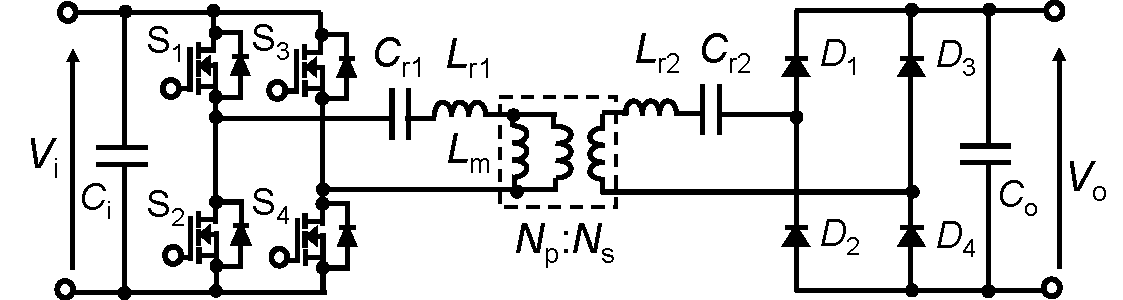
\includegraphics[width=\columnwidth]{figures_chapter5/circuitDiagram.pdf}%
        \label{fig:circuitdiagram}
    }

    \subfloat[]{
        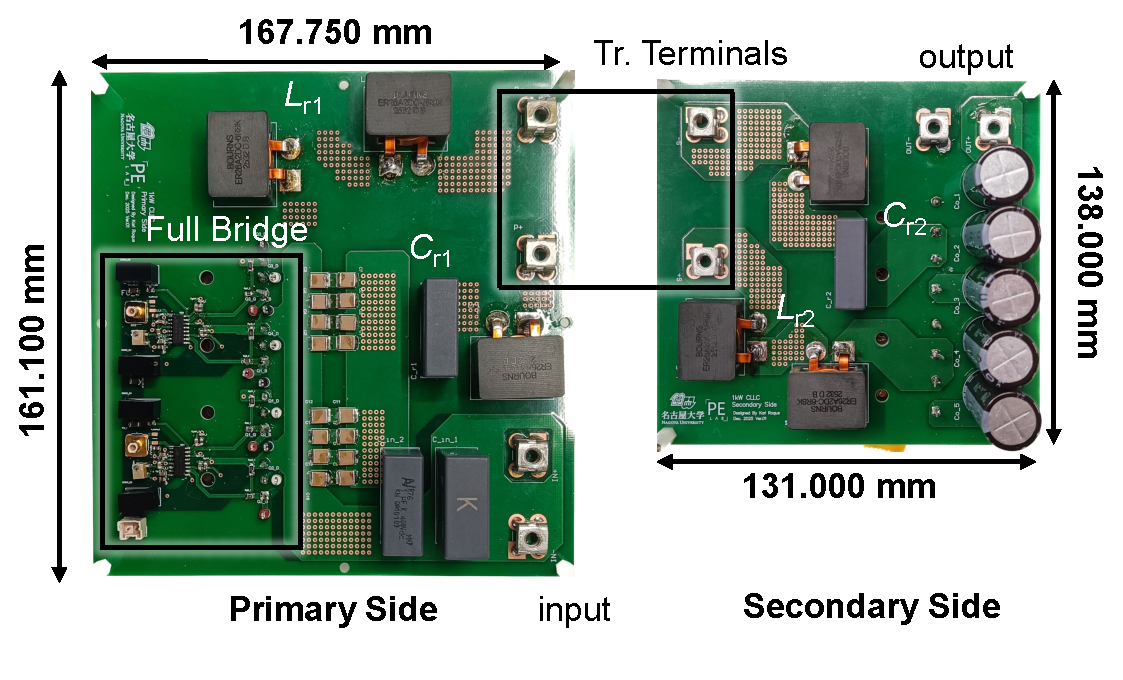
\includegraphics[width=0.8\columnwidth]{figures_chapter5/implementation_converter.pdf}
        \label{fig:converter}
    }
    \caption{(a) Circuit diagram of the manufactured 1-kW CLLC converter, (b) Photograph of the manufactured 1-kW CLLC converter.}
    \label{fig6}
\end{figure}
\begin{table}[h!]
\centering
\caption{Specifications and Components of the CLLC Resonant Converter Prototype}

\setlength{\tabcolsep}{3pt}
\resizebox{\textwidth}{!}{
\begin{tabular}{lcc}
\hline
\hline
\textbf{Parameter / Component} & \textbf{Symbol} & \textbf{Value / Part Number} \\
\hline
Input Voltage & $V_{\mathrm{i}}$ & 100 V \\
Output Voltage & $V_{\mathrm{o}}$ & 100 V \\
Maximum Rated Power & $P_{\mathrm{o}}$ & 1000 W \\
Switching Frequency & $f_{\mathrm{sw}}$ & 28.5 kHz \\
Resonant Frequency & $f_{\mathrm{r}}$ & 30.0 kHz \\
Dead Time & $t_\mathrm{d}$ & 360 ns\\
\hline
MOSFETs & $S_1, S_2, S_3, S_4$ & IPW65R050CFD7AXKSA1 \\
Half-Bridge Gate Driver & -- & SI8274GB4D-IS1 \\
Resonant Capacitors & $C_{\mathrm{r1}}, C_{\mathrm{r2}}$ & 1.4 $\upmu$F C4AQQBU4140M1WJ \\
Resonant Inductors & $L_{\mathrm{r1}}, L_{\mathrm{r2}}$ & 6.7 $\upmu$H ($\times 3$ in series) ER26A3DC-100K \\
Input Capacitors & $C_{\mathrm{in}}$ & \makecell{10 $\upmu$F R60MR51005040K \\ 1 $\upmu$F R76MR4100SE40K (in parallel)} \\
Secondary Side Diodes & $D_1, D_2, D_3, D_4$ & VX60202PW-M3/P \\
Output Capacitors & $C_{\mathrm{o}}$ & 100 $\upmu$F ($\times 5$ in parallel) 400HXW100MEFR12.5X40 \\
\hline
\hline
\end{tabular}%
}
\label{tab:prototype_components}


\end{table}

The experimental environment is shown in Figure \ref{fig:environment}. The transformer could have been isolated in a temperature-controlled environment, but this setup is chosen to mirror the possible set-up in the real-world application of the transformer. However, to isolate the thermal evaluation of the proposed transformers, the device under test (DUT) and its cooling system is put as far away as possible from the converter. An implementation of the natural and forced-air cooling scenario is shown in Figure \ref{fig:naturalaircooling} and \ref{fig:forcedaircooling} respectively.

\begin{figure}[h!]
    \centering
    
        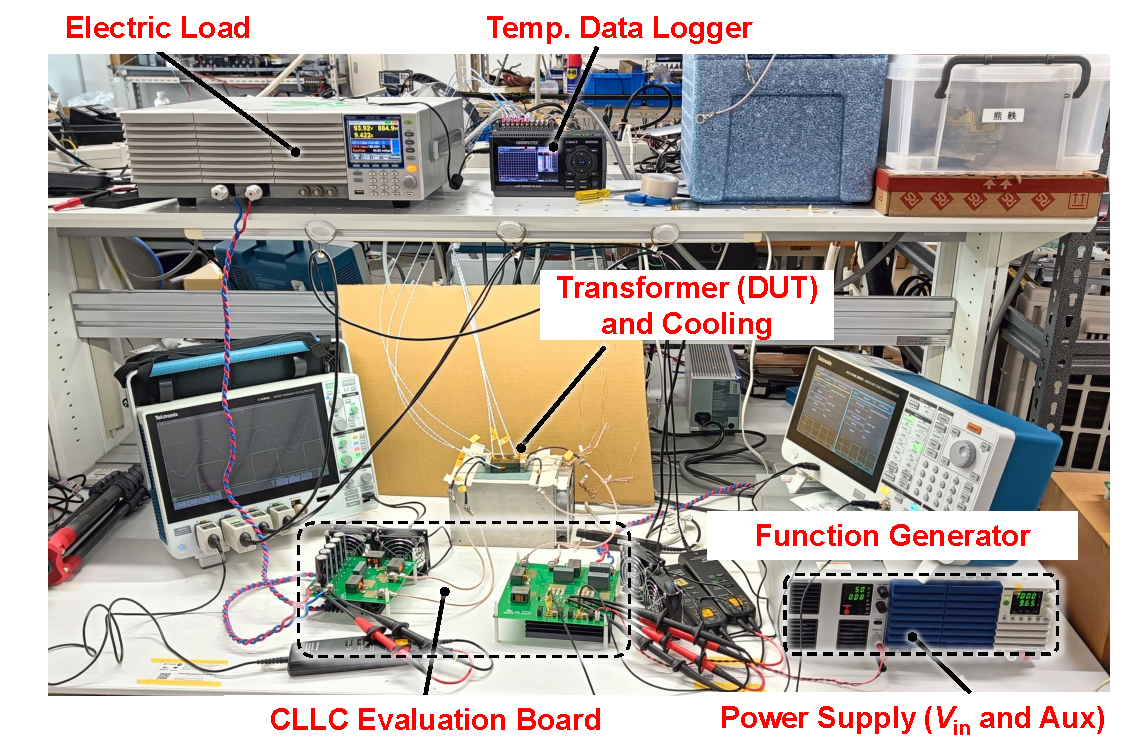
\includegraphics[width=\columnwidth]{figures_chapter5/implementation_workbench.pdf}%
        
    \caption{Experimental environment during the operational testing.}
    \label{fig:environment}
\end{figure}

\begin{figure}[h!]
    \centering
    \subfloat[]{
        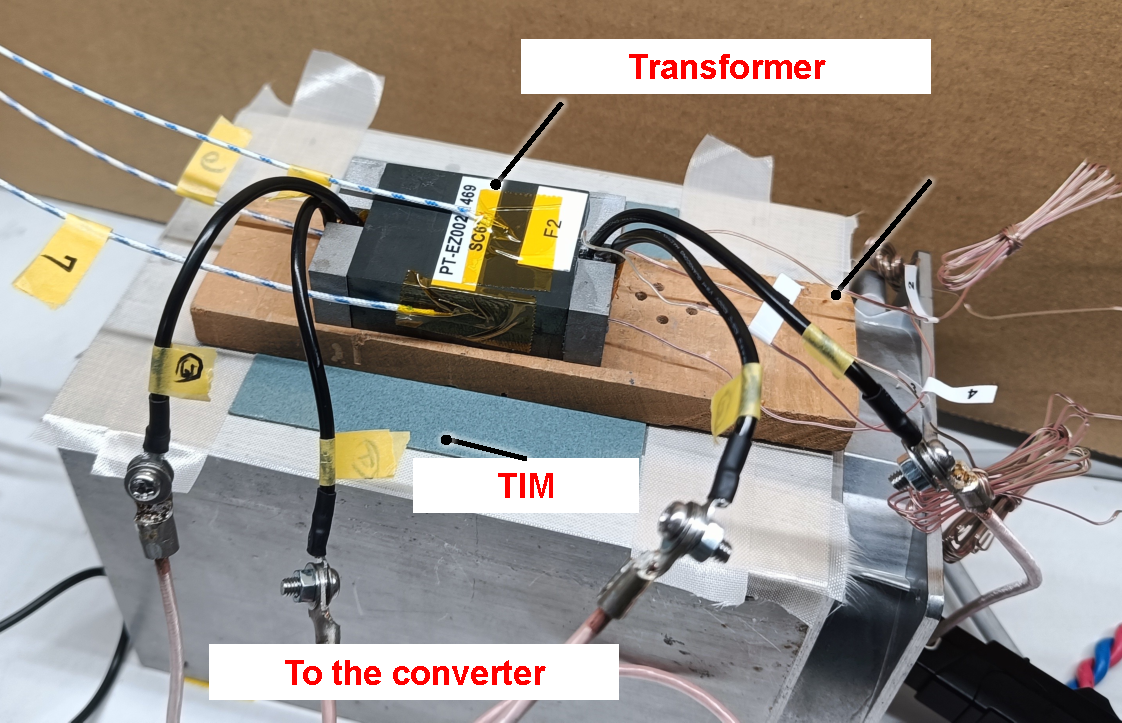
\includegraphics[width=0.7\columnwidth]{figures_chapter5/implementation_natralAir.pdf}%
        \label{fig:naturalaircooling}
    }

    \subfloat[]{
        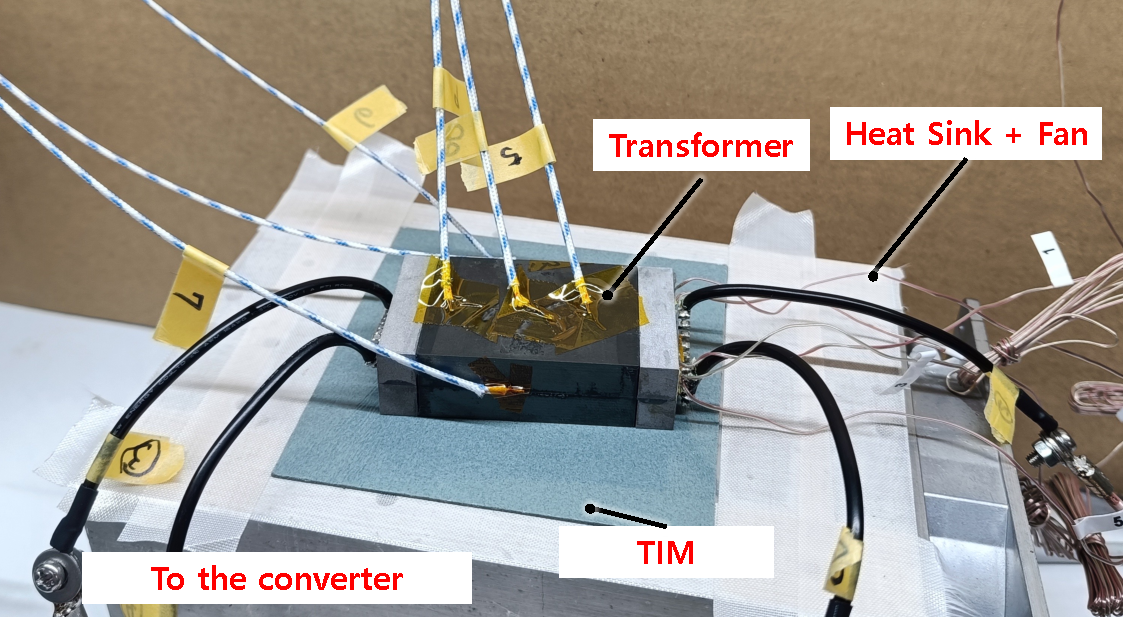
\includegraphics[width=0.7\columnwidth]{figures_chapter5/implementation_forcedAir.pdf}
        \label{fig:forcedaircooling}
    }
    \caption{Implementation of the cooling scenarios: (a) natural cooling, (b) forced-air cooling through heat sink.}
    \label{fig:imp}
\end{figure}


 Moreover, the equivalent AC resistance of each transformer was measured up to 300 kHz using a Keysight E4990A impedance analyzer from the primary side, with the secondary terminals shorted \cite{ref25}. The efficiency was also measured using a Hioki PW8001 Power Analyzer at intervals of 100 W from 100 to 1000 W. All equipment used in the experiment are detailed in Table \ref{tab:equipment}.

 \begin{table}[h!]
\centering
\caption{List of Equipment Used in the Experimental Setup}

\setlength{\tabcolsep}{3pt}
\begin{tabular}{ll}
\hline
\hline
\textbf{Equipment} & \textbf{Model / Manufacturer} \\
\hline
Oscilloscope & Tektronix MDO34 \\
Electric Load & Texio LSG-1050H \\
Function Generator & Tektronix AFG31102 \\
Power Analyzer & Hioki PW8001 + Hioki CT6841A\\
DC Power Supply & Kikusui PWR1201MH \\
AUX Power Supply (5V) & Matsusada TB160V15A720W \\
Differential Voltage Probe & Tektronix THDP0200 \\
Current Probe & Tektronix TCP0030A \\
\hline
\hline
\end{tabular}%

\label{tab:equipment}


\end{table}
 
\pagebreak
\section{Experimental Results}  
\subsection{AC Resistance Measurement Results}
Figure \ref{fig:ACResult} shows the prototype AC resistance profiles up to 300 kHz. At the operating frequency, the edgewise-wound transformer has a resistance of 32.47 m$\Omega$ while the flatwise-wound transformer has a resistance of 26.44 m$\Omega$. It seemed that the flatwise-wound transformer performed better in higher frequencies, but it is still inconclusive as the two transformers were not manufactured in exactly the same way. Further analysis is needed to quantify the winding loss performance of the two configurations. 
\begin{figure}[h!]
            \centering
            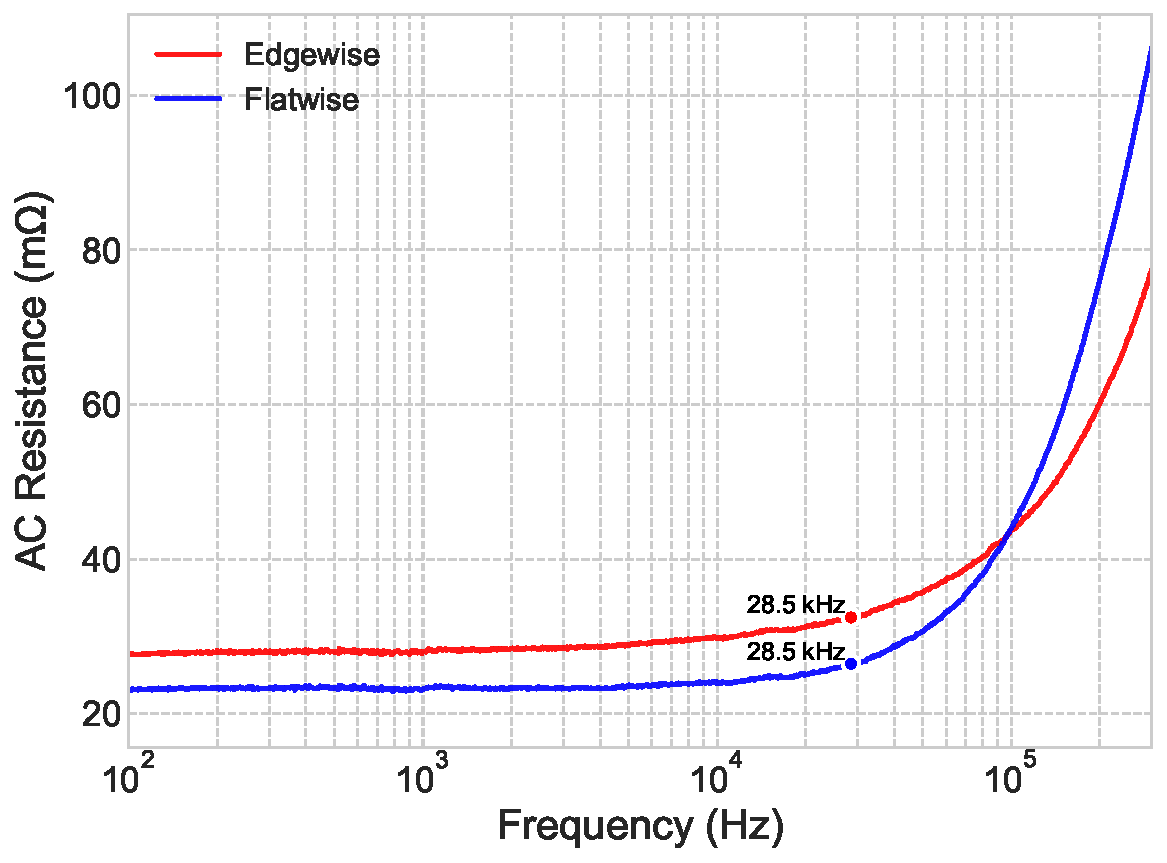
\includegraphics[width=0.7\columnwidth]{figures_chapter5/rs_short_circuit.pdf}
    \caption{AC Resistance profiles up to 300 kHz for the constructed prototypes.}
    \label{fig:ACResult}
\end{figure}
\pagebreak
\subsection{Operational Waveforms}
The zero-voltage switching (ZVS) experimental waveforms for the 1~kW CLLC converter operating at a 28.5~kHz switching frequency under natural and forced-air cooling are shown in Figure~\ref{fig:15}. Figure~\ref{fig:15a} and Figure~\ref{fig:15b} show the waveforms for the edgewise-wound and flatwise-wound transformer under natural cooling. Figure~\ref{fig:15c} and Figure~\ref{fig:15d} show the waveforms for the edgewise-wound and flatwise-wound transformer under forced-air cooling. Both the edgewise-wound and flatwise-wound prototypes demonstrate stable operation, with the primary side resonant current $i_{{\mathrm{r}_{\mathrm{pri}}}}$, output voltage $V_\mathrm{O}$, high-side gate voltage $V_\mathrm{gs}$, and drain-to-source voltage $V_\mathrm{ds}$ remaining well-regulated across both cooling conditions.
 
\begin{figure}[H]
\centering
% (a) Top circuit
        \subfloat[]{
        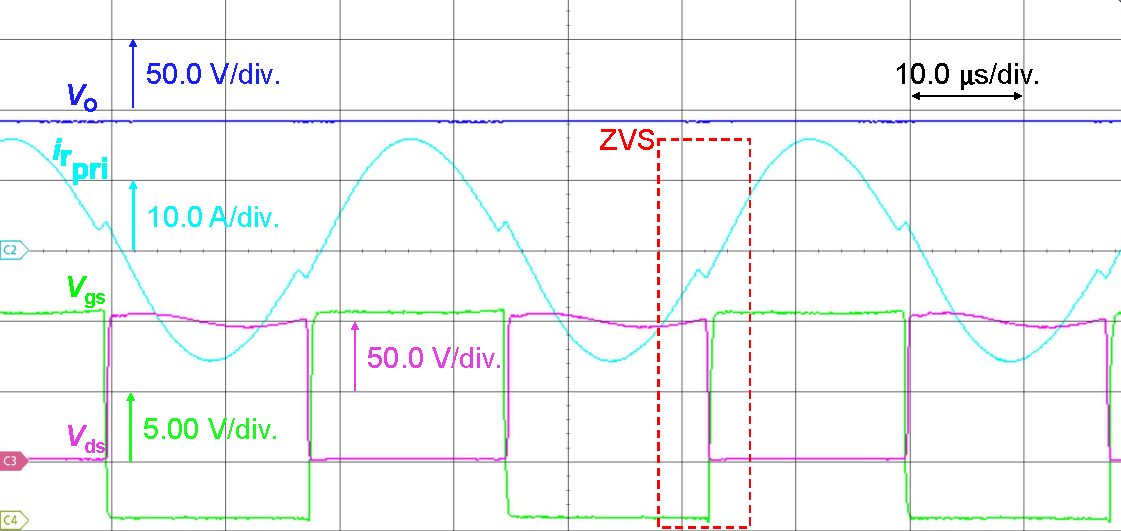
\includegraphics[width=0.7\columnwidth]{figures_chapter5/E2_natural.pdf} % Make sure this file exists
        \label{fig:15a}
        } 
        % This double backslash forces the next image to the line below (vertical stack)
        % (b) Middle circuit

        \subfloat[]{
        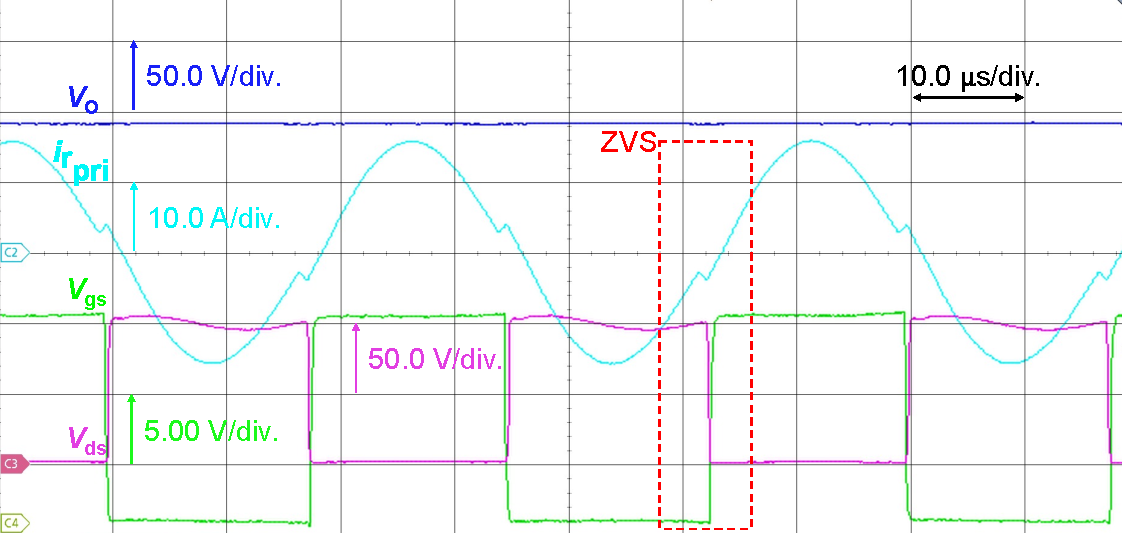
\includegraphics[width=0.7\columnwidth]{figures_chapter5/F2_natural.pdf}
        \label{fig:15b}
        }

        \subfloat[]{
        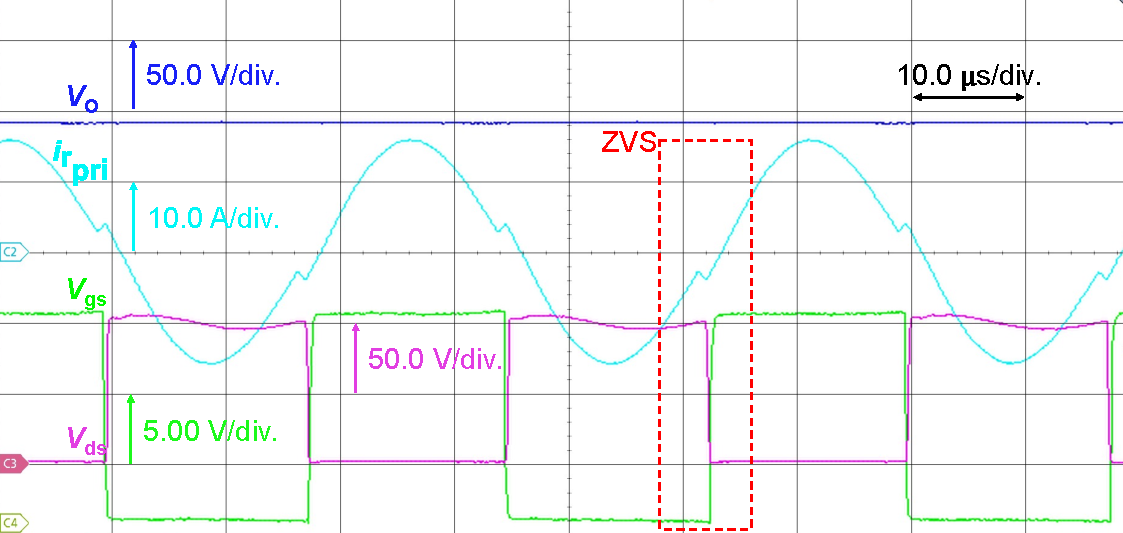
\includegraphics[width=0.7\columnwidth]{figures_chapter5/E2_forced.pdf} % Make sure this file exists
        \label{fig:15c}
        } 
        
        \subfloat[]{
        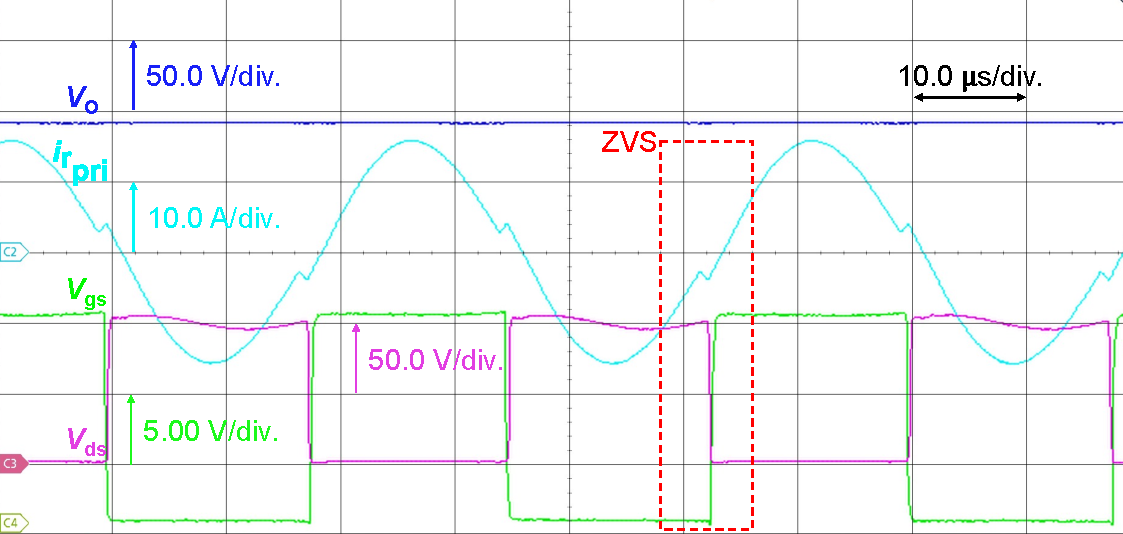
\includegraphics[width=0.7\columnwidth]{figures_chapter5/F2_forcedair.pdf}
        \label{fig:15d}
        } 
        \caption{Experimental waveforms of the transformers implemented in a 1-kW, 28.5-kHz CLLC at natural cooling: (a) edgewise-wound transformer, (b) flatwise-wound transformer; and forced-air cooling: (c) edgewise-wound transformer, (d) flatwise-wound transformer.}
        \label{fig:15}
\end{figure}

\pagebreak
\subsection{Temperature Profiles}
The measured temperature profiles of the edgewise and flatwise transformers during natural cooling are shown in Figure~\ref{fig:18}a and Figure~\ref{fig:18}b. As shown in the edgewise thermal profile, the temperature curve did not stabilize after one hour of continuous operation. To prevent thermal runaway, the test was aborted, recording a peak transient $T_{\mathrm{wind}}$ of 74.3$^{\circ}$C. The test for the flatwise transformer was also recorded for one hour and was able to stabilize at $T_{\mathrm{wind}}$ of 66.7$^{\circ}$C. Longer full-load results are available through a repeat test as shown in the Appendix: \nameref{app:longresult}.

In the natural cooling evaluation, both prototypes exhibited tight thermal coupling between the primary winding and the internal core window, shown by a 0.8 to 1.3$^{\circ}$C gradient between $T_{\mathrm{wind}}$ and $T_{\mathrm{top, in}}$, $T_{\mathrm{left, in}}$. However, in terms of the internal-to-external temperature gradient, the edgewise structure suffers from a 9.0$^{\circ}$C gradient between $T_{\mathrm{wind}}$ and $T_{\mathrm{top, out}}$, and a 13.4$^{\circ}$C gradient to $T_{\mathrm{left, out}}$, indicating internal heat entrapment. The flatwise structure reduces these internal-to-external gradients to 4.1$^{\circ}$C and 8.7$^{\circ}$C, respectively. This therefore proves that the flatwise structure is able to move heat easily from the inside to the outside, preventing heat from getting trapped inside the core.

Furthermore, the observed temperature hierarchy, indicated by $T_{\mathrm{wind}} > T_{\mathrm{top, in}}$, $T_{\mathrm{left, in}} > T_{\mathrm{top, out}} > T_{\mathrm{left, out}}$ aligns with the fundamental heat transfer mechanisms of the transformer. The internal winding serves as the primary heat source, leading to $T_{\mathrm{wind}}$ peaking. Consequently, $T_{\mathrm{top, in}}$, $T_{\mathrm{left, in}}$ maintain elevated temperatures necessary to overcome the thermal resistance of the ferrite core and facilitate outward conduction. At the exterior boundaries, the cooling efficiency is governed by natural convection. Heat dissipation at the top horizontal surface is constrained by the upward plume of heated air, which reduces the local convective heat transfer coefficient. Conversely, the vertical outer leg is exposed to a continuous buoyancy-driven flow of cooler ambient air. This then leads to $T_{\mathrm{top, out}} > T_{\mathrm{left, out}}$.

The advantage of the flatwise structure is further demonstrated during the forced-air cooling evaluation. Under forced-air cooling, the temperature profiles shown in Figure~\ref{fig:18}c and Figure~\ref{fig:18}d confirm that both prototypes reached a stable steady state. However, the edgewise $T_{\mathrm{wind}}$ stabilized at a higher temperature of 46.5$^{\circ}$C, whereas the flatwise $T_{\mathrm{wind}}$ maintained a cooler steady-state operating temperature of 41.5$^{\circ}$C. 

The active cooling system anchored $T_{\mathrm{bot, out}}$ at 31.1$^{\circ}$C and 31.3$^{\circ}$C for the edgewise and flatwise structures, respectively. The $T_{\mathrm{top, out}}$ for both structures was approximately 40.0$^{\circ}$C. However, the internal thermal distribution shows a clear difference in thermal resistance. The edgewise prototype had a 15.4$^{\circ}$C gradient between $T_{\mathrm{wind}}$ and $T_{\mathrm{bot, out}}$, and a 6.6$^{\circ}$C gradient between $T_{\mathrm{wind}}$ and $T_{\mathrm{top, out}}$. The flatwise prototype had a 10.2$^{\circ}$C gradient and a 1.3$^{\circ}$C gradient between $T_{\mathrm{wind}}$ and $T_{\mathrm{bot, out}}$, and $T_{\mathrm{top, out}}$, respectively. Additionally, the gradient between $T_{\mathrm{wind}}$ and $T_{\mathrm{Al}}$ was 3.4$^{\circ}$C for the flatwise prototype, compared to 5.7$^{\circ}$C for the edgewise prototype. Because the flatwise exterior temperatures closely match its interior winding temperature, these gradients prove the thermal advantage of the flatwise structure.

To summarize, with the flatwise-wound prototype, the peak winding temperature was reduced by 7.7$^{\circ}$C in natural cooling and 5.0$^{\circ}$C in forced air cooling. Moreover, the temperature gradients $T_{\mathrm{wind}} - T_{\mathrm{top, out}}$ and $T_{\mathrm{wind}} - T_{\mathrm{bot, out}}$ were reduced by 4.9$^{\circ}$C and 3.4$^{\circ}$C respectively under natural cooling conditions, and 5.2$^{\circ}$C and 5.3$^{\circ}$C respectively under forced-air cooling conditions.
\pagebreak
\begin{figure}[h!]
\centering
% (a) Left circuit
        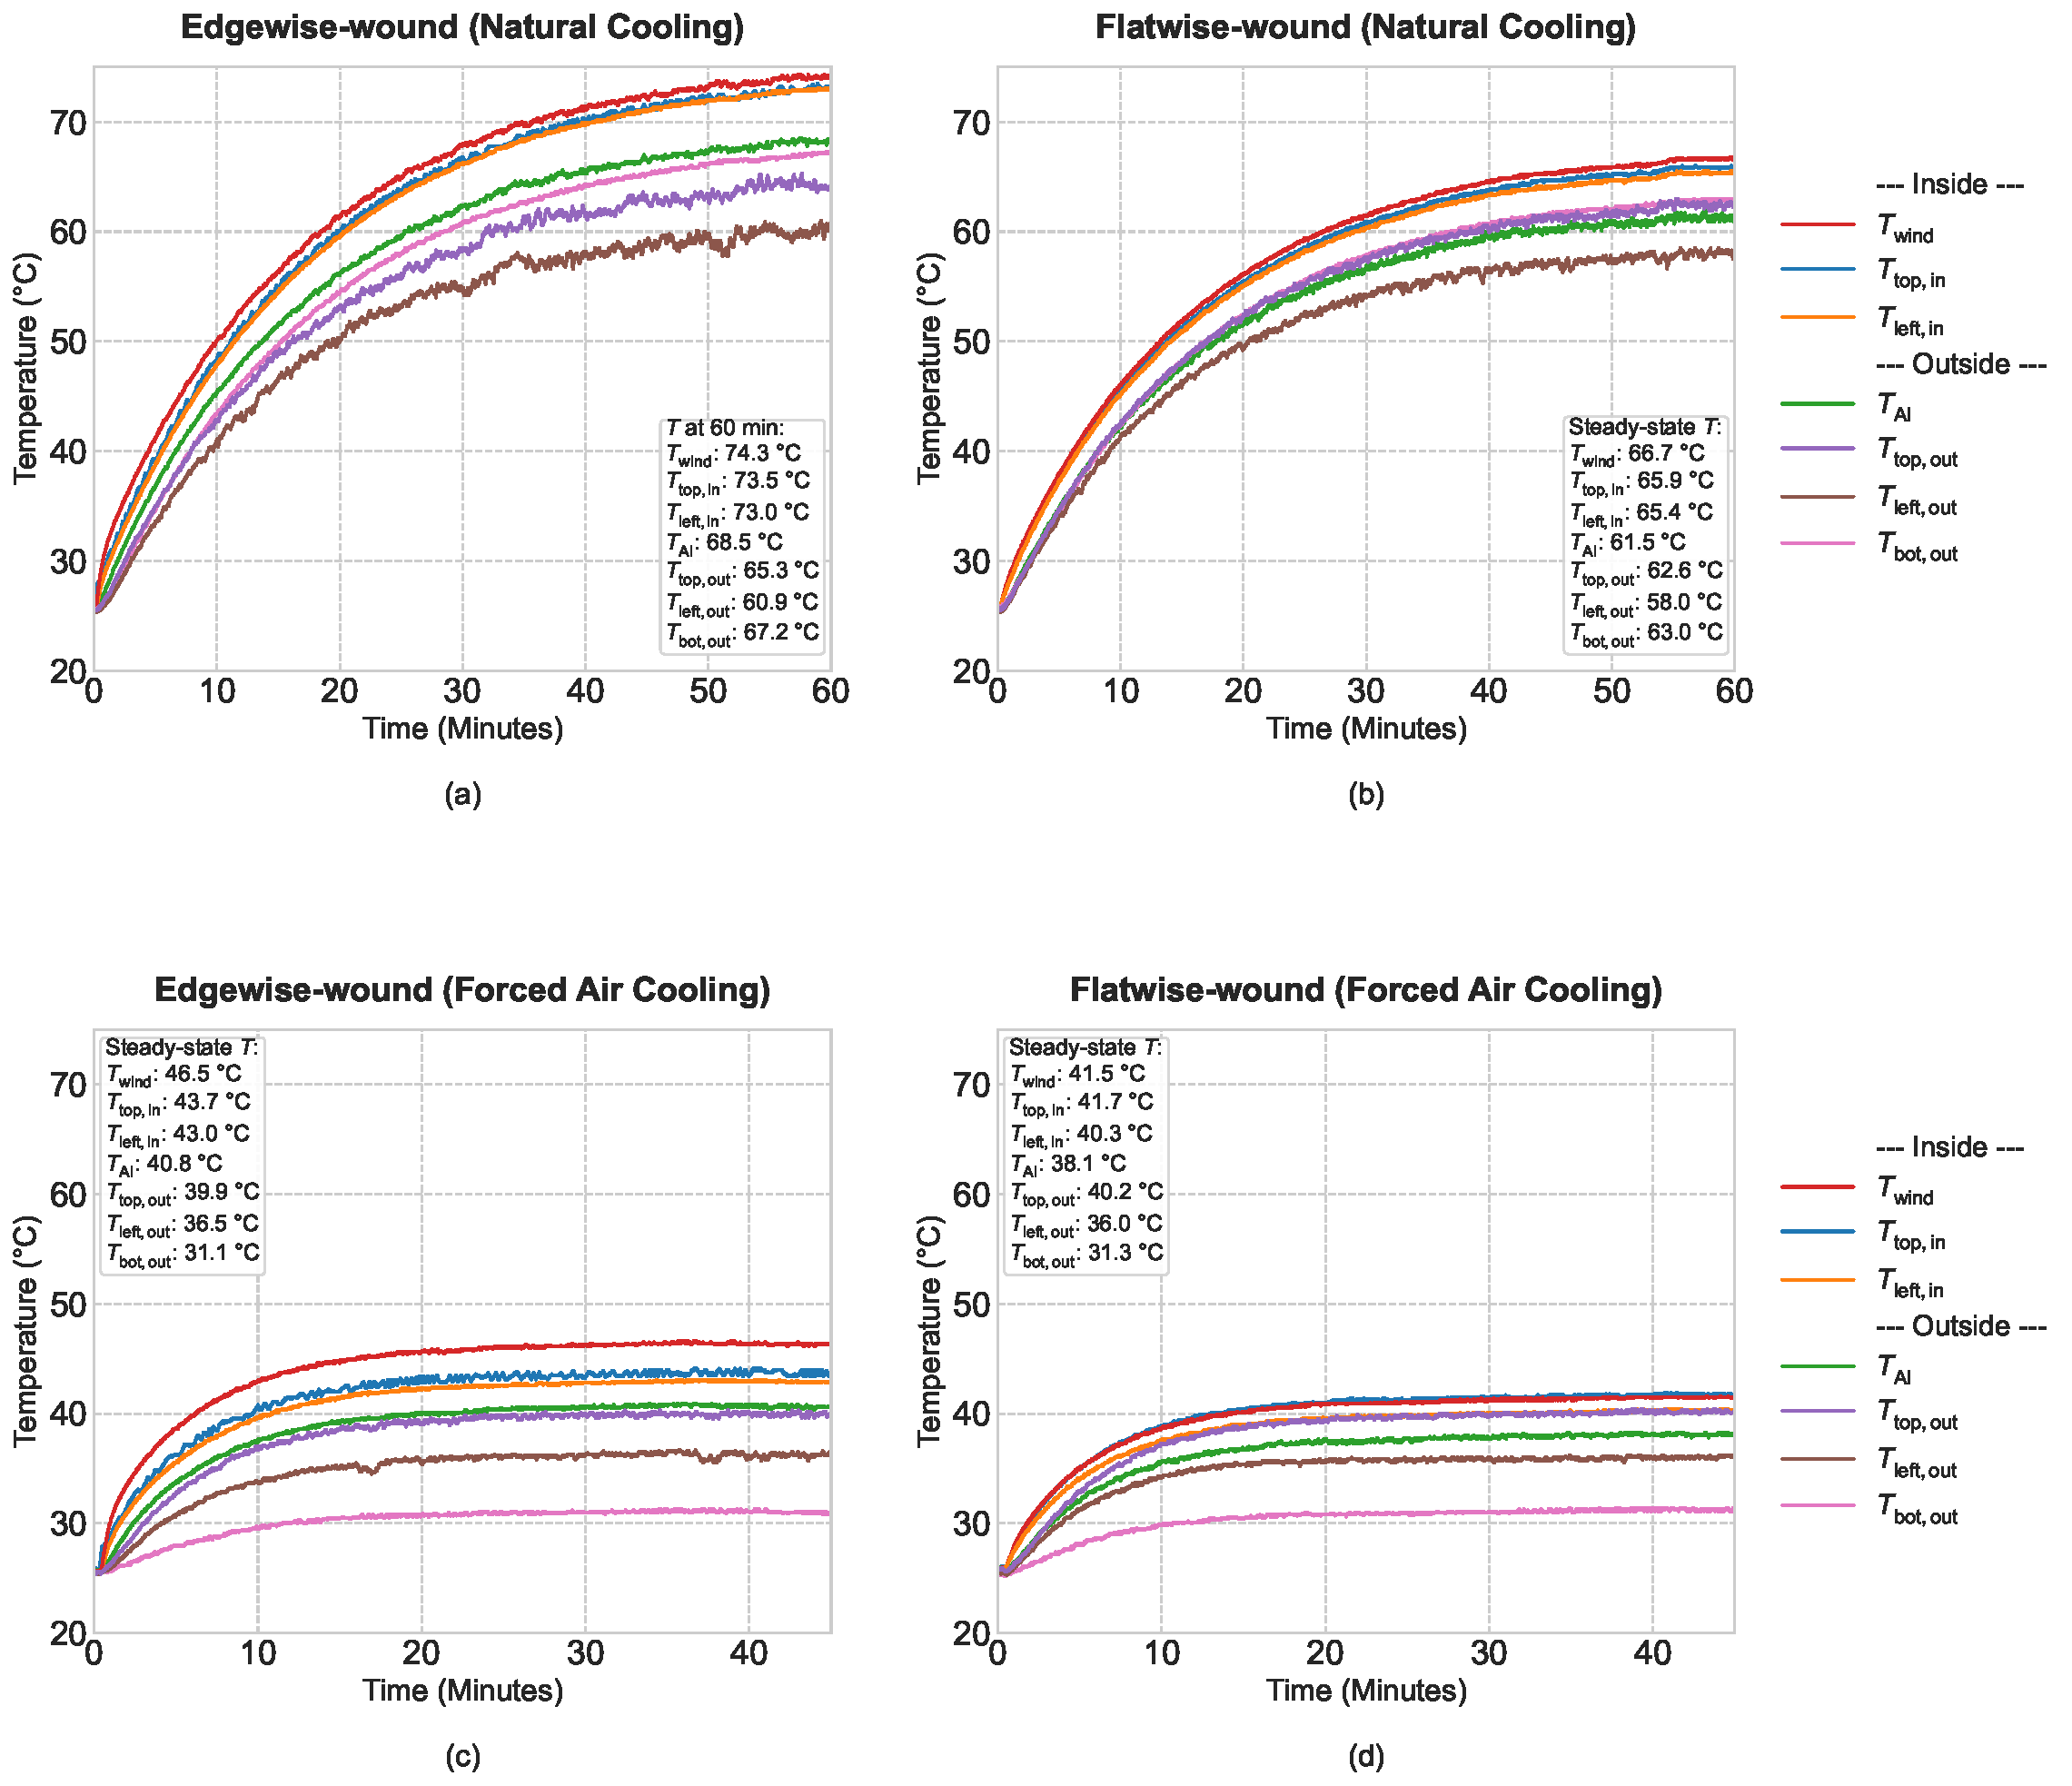
\includegraphics[width=\columnwidth]{figures_chapter5/Combined_Thermal_Comparison.pdf} 
        \caption{Temperature profiles of the transformers at natural cooling: (a) edgewise-wound transformer, (b) flatwise-wound transformer; and forced-air cooling through a heat sink: (c) edgewise-wound transformer, (d) flatwise-wound transformer.}
        \label{fig:18}
\end{figure}

%To confirm the uniformity of distribution on the surfaces of the transformer and for repeatability, the test was repeated once again. Results are shown in Figure xx.

\pagebreak
\subsection{System Efficiency}
The system-level efficiency was examined using the same 1-kW converter for each test case. An input power-efficiency curve is shown in Figure \ref{fig:eff}. The peak efficiency was observed at around 30\% or 300 W load in both cases. The full load efficiency of the system is at 92.5\%. This entails that both transformers allow for close performance, entailing no problem in using the proposed transformer. The flatwise-wound transformer is then able to guarantee superior internal-to-external thermal resistance without affecting the system-level efficiency.
\begin{figure}[h!]
\centering
% (a) Left circuit
        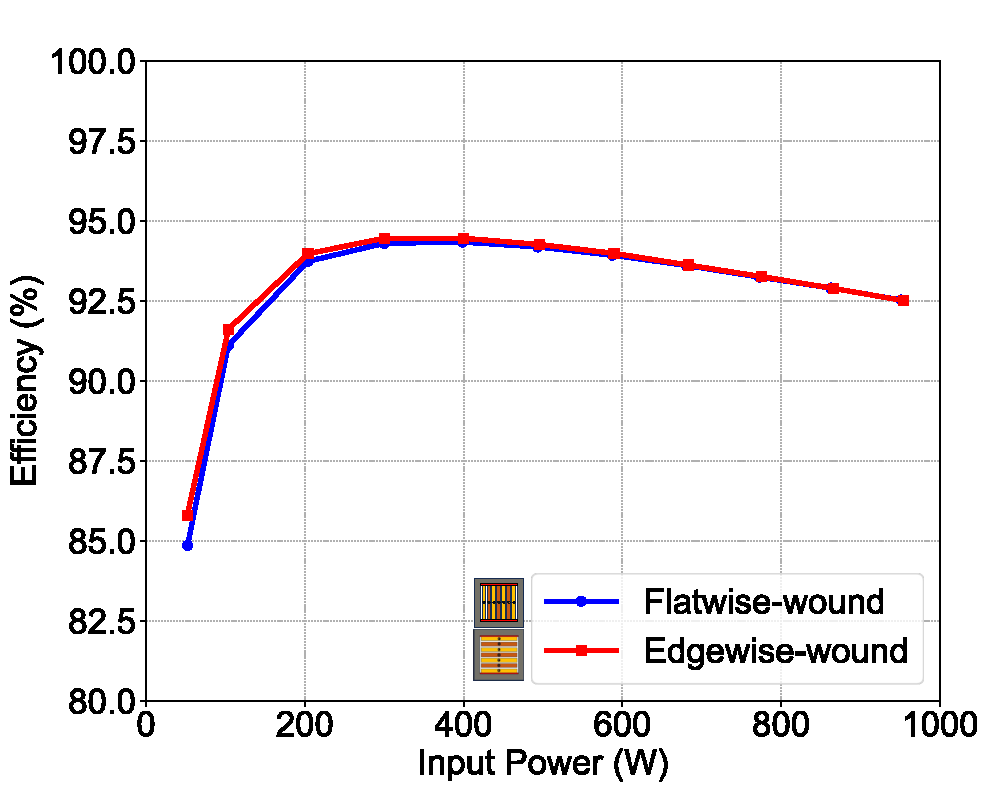
\includegraphics[width=0.7\columnwidth]{figures_chapter5/efficiency.pdf} 
        \caption{System-level efficiency of the 1-kW CLLC at 28.5 kHz operating frequency, from 50W to 1000W input power.}
        \label{fig:eff}
\end{figure}

%\subsection{Reverse Engineering Simulation}
%The simulation for the constructed prototypes were repeated once again. This time, the whole cooling setup is reproduced as close as possible in simulation. A sample of the simulation model is shown in Figure xx. 

%The 